\begin{activite}[Les rectangles]
\ImageDroite{%
\begin{enumerate}
    \item Sur ton cahier, reproduis les rectangles roses de telle sorte qu'ils forment un grand rectangle. Pourquoi peut-on les regrouper facilement ?
    \item Calcule l'aire totale des rectangles roses de deux façons différentes. (L'une d'elles ne doit comporter qu'une seule multiplication.)
    \item Reprends les deux questions précédentes pour les rectangles verts.
    \item Wilfrid affirme qu'il peut calculer la somme des aires des six rectangles en utilisant une seule multiplication. Comment fait-il ? Pourquoi est-ce possible ?
\end{enumerate}
}{\vspace*{2cm}
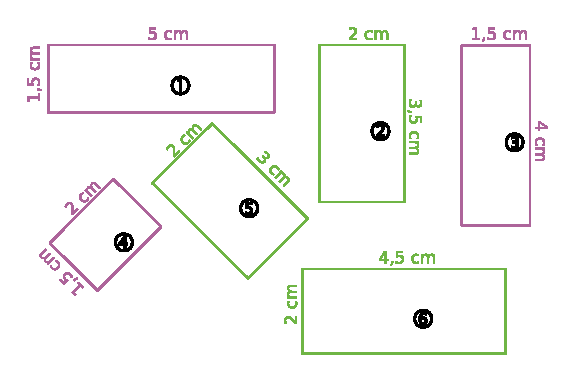
\includegraphics[width=.45\linewidth]{DiA01}}
\end{activite}
 




\begin{activite}[Avec des mots]
En lisant son cours de mathématiques sur le chapitre \og Distributivité \fg, Odile remarque qu'il existe des phénomènes très similaires dans certaines phrases.

\vspace{1em}\textbf{1\up{ère} Partie}\vspace{1em}

Odile se dit qu'on peut parfois développer le sujet ou le verbe d'une phrase. 
Par exemple : Dans la phrase \og Marius et Gaëlle mangent. \fg, on peut développer le verbe, ce qui donne : \og Marius mange et Gaëlle mange. \fg.

\begin{enumerate}
\item Développe les phrases suivantes :
\og Audrey relit et apprend ses leçons. \fg ;
\og La pluie, le vent et le froid l'empêchaient de sortir de la maison. \fg.
\item Invente une phrase de ton choix dans laquelle on peut développer le verbe.

\vspace{1em}\textbf{2\up{e} Partie}\vspace{1em}

Odile se dit qu'on peut aussi utiliser des mots mathématiques dans ces phrases.

\item Développe la phrase suivante : \og 78 et 12 sont multipliés par 5. \fg.
\end{enumerate}
\end{activite}
 







\begin{activite}[Calcul réfléchi]
Lucie connaît ses tables de multiplication jusqu'à 10 et voudrait construire la table de 11. Anthony, son voisin, lui explique que c'est facile de la trouver et lui donne un exemple à l'oral : 
\og onze fois quatorze \fg, c’est \og dix fois quatorze plus une fois quatorze \fg.
Comme Lucie n'a pas très bien compris, Anthony écrit alors :
\begin{align*}
    11 \times 14 	&= 10 \times 14 + 1 \times 14 \\
		&= 140 + 14 \\
		&= 154 \\
\end{align*}

\begin{enumerate}
    \item Écris la phrase puis le calcul pour $11 \times 15$ et $17 \times 11$.
    \item Recopie puis complète la table de 11 suivante.

\renewcommand*\tabularxcolumn[1]{>{\centering\arraybackslash}m{#1}}
\begin{lctableau}{\linewidth}{12}
\hline
$\times$ & 10 & 11 & 12 & 13 & 14 & 15 & 16 & 17 & 18 & 19 & 20 \\ \hline
11 & & & & & 154 & & & & & & \\ \hline
\end{lctableau}

    \item\label{DisAc01} Lucie propose alors de calculer $13 \times 21$ en procédant de façon similaire. Elle note ses calculs intermédiaires dans le tableau ci-dessous.

\begin{center}
\begin{minipage}[c]{.35\linewidth}
\renewcommand*\tabularxcolumn[1]{>{\centering\arraybackslash}m{#1}}
\begin{lctableau}{\linewidth}{3}
\hline
$\times$ & 20 & 1  \\ \hline
13 & 260 & 13\\ \hline
\end{lctableau}
\end{minipage}
\end{center}

Elle obtient : $13 \times 21 = 273$.

Explique comment elle a obtenu 273 comme résultat.

    \item Calcule les produits suivants en présentant les résultats intermédiaires dans un tableau.
        \subitem $12 \times 34$
        \subitem $17 \times 1 001$
    \item Anthony fait remarquer que l'on peut aussi calculer facilement $13 \times 19$ à partir des résultats intermédiaires notés dans le tableau. Calcule ce produit.
    \item Avec les tableaux que tu as construits à la question \ref{DisAc01}, quels autres produits peux-tu calculer facilement ? Écris-les puis calcule-les.
\end{enumerate}
\end{activite}





\begin{activite}[Développer $(a + b)(c + d)$]
\begin{enumerate}
    \item On considère le produit $P = 86 \times 53$. Justifie les égalités suivantes : $P = 86 \times 50 + 86 \times 3$ puis $P = 80 \times 50 + 6 \times 50 + 80 \times 3 + 6 \times 3$.

Déduis-en l'égalité : $(80 + 6) \times (50 + 3) = 80 \times 50 + 6 \times 50 + 80 \times 3 + 6 \times 3$ puis calcule $P$ sans poser de multiplication (et sans calculatrice !).
    \item Complète : $(a + b)(c + d) = ... \times (c + d) + ... \times (c + d) = ... + ... + ... + ...$.
    
Quelle propriété as-tu utilisée ? Combien de fois ? En quoi a été transformé le produit initial ?
    \item \subitem a) Complète : $(3x  - 2)(5x + 4) = (... + ...) \times (... + ...)$.
    \subitem b) Déduis-en le développement de ce produit.
    \subitem c) Procède de même avec le produit $(2  - y)(2y  - 5)$.
    \item Pour développer le produit $(2a + 3)(3a  - 4)$, on peut poser la multiplication comme indiqué ci-dessous.
    
    \begin{center}
        
\includegraphics[width=.33\linewidth]{DiA02}
    \end{center}
    
    Effectue-la sans oublier le décalage.
\end{enumerate}
\end{activite}
